\onecolumngrid
\setcounter{figure}{0}
\setcounter{table}{0}
\renewcommand{\thefigure}{S\arabic{figure}}
\renewcommand{\thetable}{S\Roman{table}}

\subsection*{Supplemental Tables and Figures}

% Table generated by Excel2LaTeX from sheet 'Sheet1'
\begin{table}[htbp]
  \centering
  \caption{Focus reduction assay of reference viruses and contemporary test viruses.}
    \begin{tabular}{|p{11em}|p{3em}|r|r|p{5em}|r|}
    \toprule
    \multicolumn{2}{c|}{\multirow{3}[3]{*}{}} & \multicolumn{4}{p{20em}|}{\textbf{Reference Ferret Antisera}} \\
\cmidrule{3-6}    \multicolumn{2}{c|}{} & \multicolumn{1}{p{5em}|}{A/Michigan} & \multicolumn{1}{p{5em}|}{A/Singapore} & A/Nebraska & \multicolumn{1}{p{5em}|}{A/California} \\
    \multicolumn{2}{c|}{} & \multicolumn{1}{p{5em}|}{/15/2014} & \multicolumn{1}{p{5em}|}{/INFIMH-16-0019/2016} & /2/2017 & \multicolumn{1}{p{5em}|}{/179/2016} \\
    \textbf{Reference Virus} & \textbf{Clade} & \multicolumn{1}{p{5em}|}{\cellcolor[rgb]{ .282,  .439,  .922}3c2.A} & \multicolumn{1}{p{5em}|}{\cellcolor[rgb]{ .459,  .776,  .663}A1} & \cellcolor[rgb]{ .996,  .733,  .263}A2 & \multicolumn{1}{p{5em}|}{\cellcolor[rgb]{ 1,  .412,  .2}A3} \\
    \midrule
    A/Michigan/15/2014 & \cellcolor[rgb]{ .282,  .439,  .922}3c2.A & \textbf{640} & 320   & \multicolumn{1}{r|}{1600} & 320 \\
    A/Singapore/Infimh-16-0019/16 & \cellcolor[rgb]{ .459,  .776,  .663}A1 & 640   & \textbf{1280} & \multicolumn{1}{r|}{800} & 1280 \\
    A/Nebraska/02/2017 & \cellcolor[rgb]{ .996,  .733,  .263}A2 & 640   & 1280  & \multicolumn{1}{r|}{\textbf{12800}} & 1280 \\
    \midrule
    A/California/179/2016 & \cellcolor[rgb]{ 1,  .412,  .2}A3 & 640   & 2560  & \multicolumn{1}{r|}{800} & \textbf{1280} \\
    \midrule
    \textbf{Test Virus} & \multicolumn{5}{c|}{} \\
    \midrule
    A/Haiti/5464/2017 & \cellcolor[rgb]{ .678,  .839,  .416}A1b & 640   & 1280  & \multicolumn{1}{r|}{1600} & 1280 \\
    \midrule
    A/Maryland/13/2018 & \cellcolor[rgb]{ .678,  .839,  .416}A1b & 320   & 1280  & \multicolumn{1}{r|}{400} & 640 \\
    \midrule
    A/Kuwait/922/2018 & \cellcolor[rgb]{ .678,  .839,  .416}A1b & 320   & 1280  & \multicolumn{1}{r|}{400} & 640 \\
    A/Kazakhstan/079/2018 & \cellcolor[rgb]{ .996,  .733,  .263}A2 & 640   & 1280  & \multicolumn{1}{r|}{12800} & 640 \\
    \midrule
    A/Kazakhstan/031/2018 & \cellcolor[rgb]{ .996,  .733,  .263}A2 & 640   & 640   & \multicolumn{1}{r|}{12800} & 1280 \\
    \midrule
    A/Alberta/Rv2371/2017 & \cellcolor[rgb]{ .996,  .733,  .263}A2 & 320   & 640   & \multicolumn{1}{r|}{6400} & 640 \\
    \midrule
    A/Tennessee/70/2017 & \cellcolor[rgb]{ 1,  .6,  .231}A2/re & 640   & 2560  & \multicolumn{1}{r|}{25600} & 1280 \\
    \midrule
    A/Puerto Rico/09/2018 & \cellcolor[rgb]{ 1,  .6,  .231}A2/re & 640   & 2560  & \multicolumn{1}{r|}{25600} & 1280 \\
    \midrule
    A/Peru/3817/2017 & \cellcolor[rgb]{ 1,  .6,  .231}A2/re & 640   & 640   & \multicolumn{1}{r|}{12800} & 640 \\
    A/Cambodia/949/2017 & \cellcolor[rgb]{ 1,  .412,  .2}A3 & 320   & 640   & \multicolumn{1}{r|}{800} & 640 \\
    A/New Jersey/23/2018 & \cellcolor[rgb]{ .38,  .702,  .788}3c3.A & 80    & 320   & \multicolumn{1}{r|}{\textless200}  & 80 \\
    \midrule
    A/Delaware/20/2018 & \cellcolor[rgb]{ .38,  .702,  .788}3c3.A & 20    & 160   & \multicolumn{1}{r|}{\textless200}  & 40 \\
    \midrule
    A/Massachusetts/18/2018 & \cellcolor[rgb]{ .38,  .702,  .788}3c3.A & 40    & 80    & \multicolumn{1}{r|}{\textless200}  & 40 \\
    \bottomrule
    \end{tabular}%
  \label{sup_tab:titer_table}%
\end{table}%


\begin{figure*}[h]
    \begin{center}
    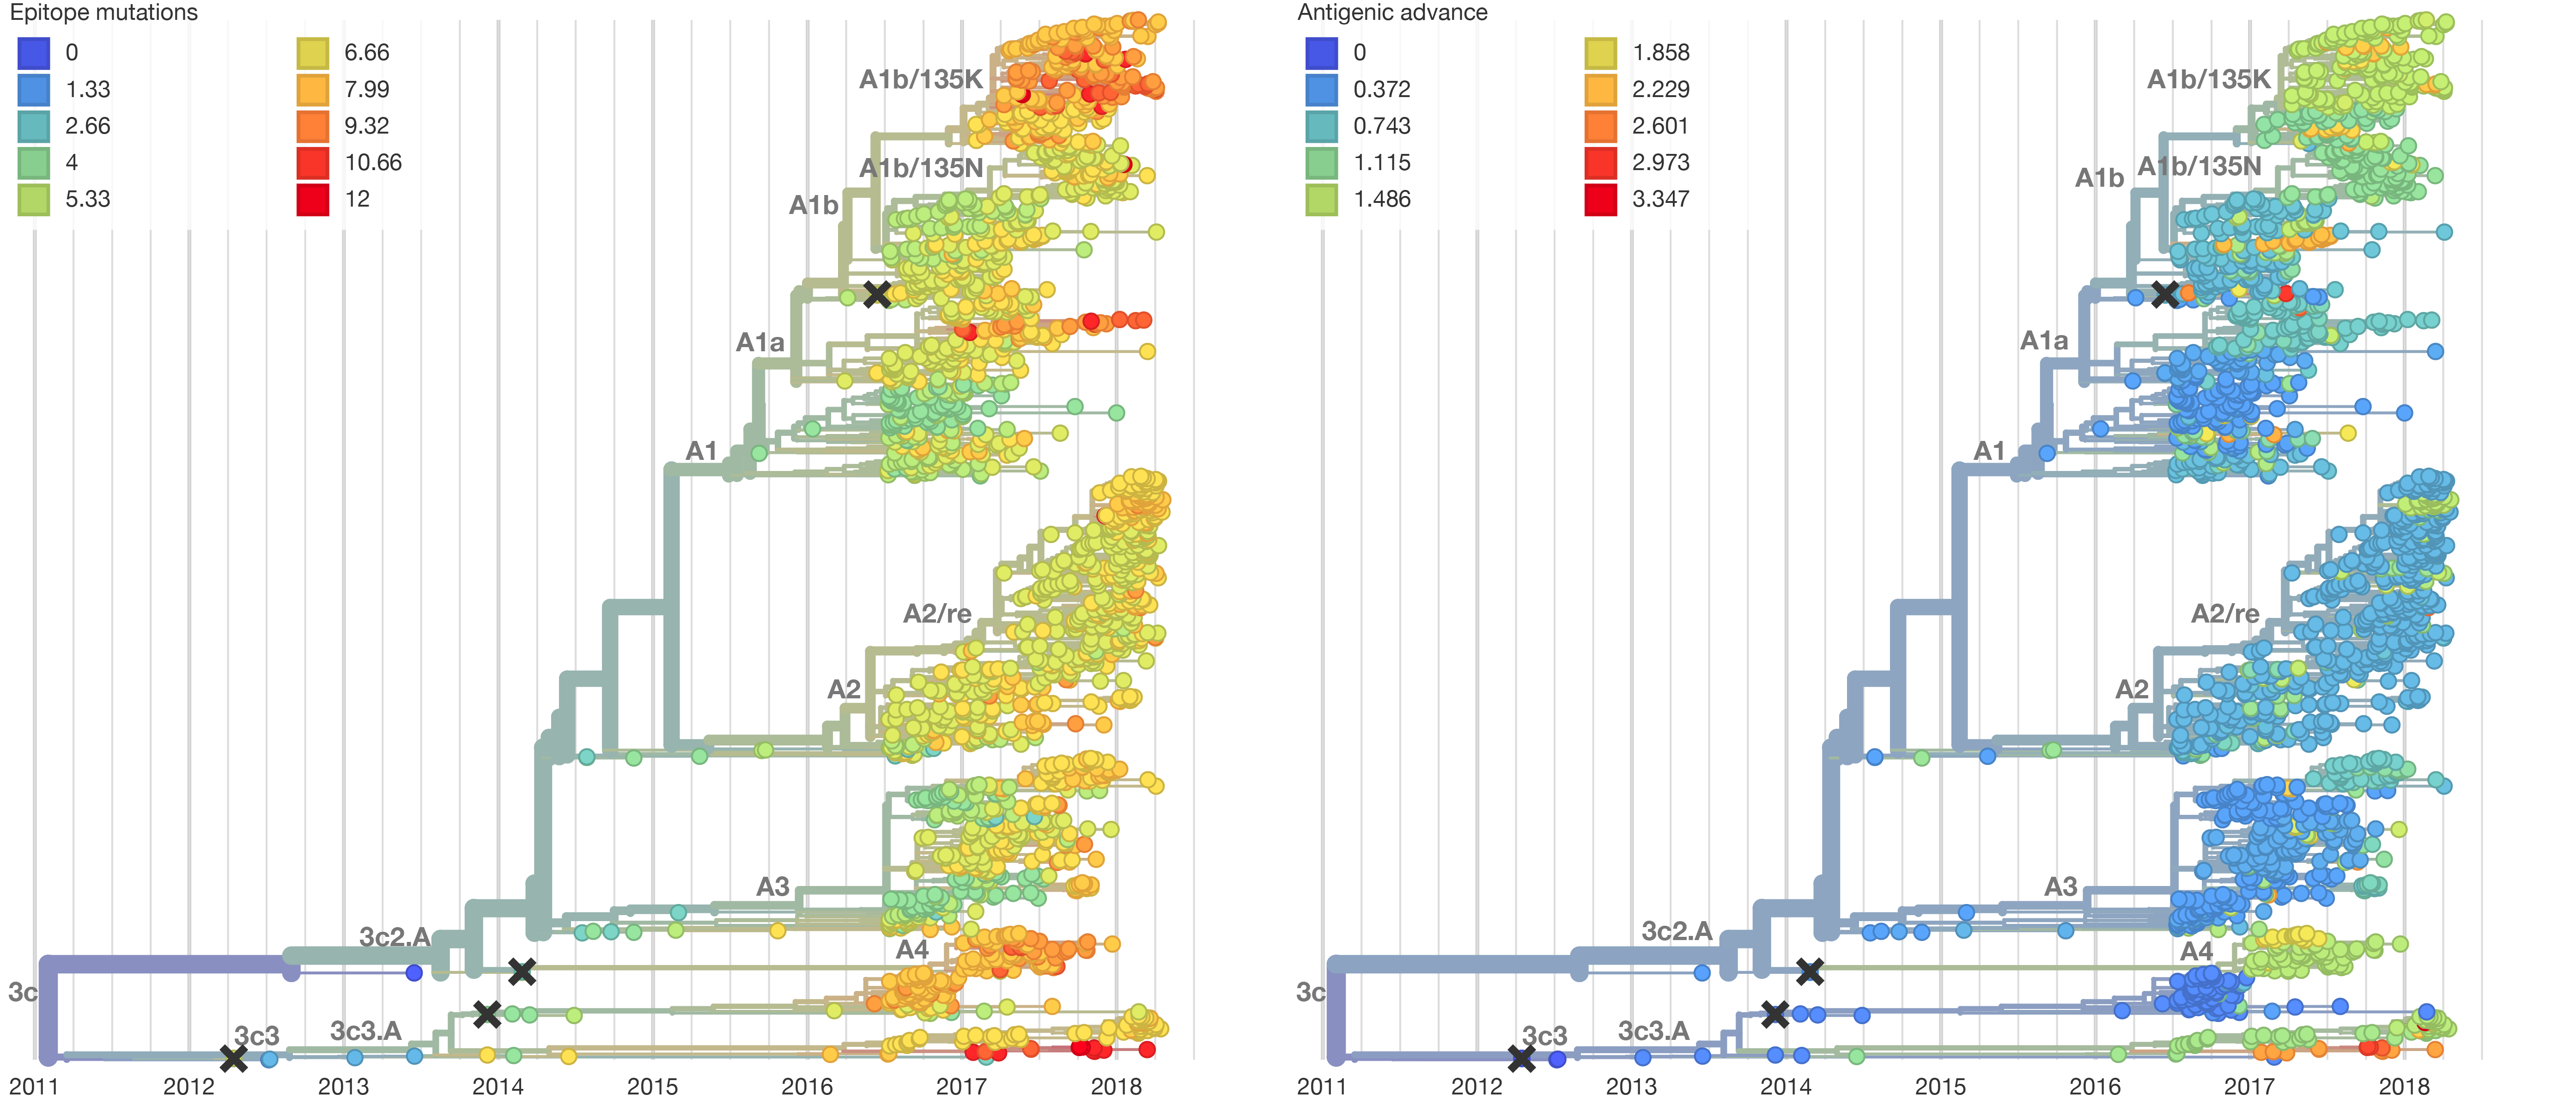
\includegraphics[width=\textwidth]{figures/epi_aa_trees_high_res.png}
    \end{center}
    \caption{\textit{(left)} Temporally resolved haemagglutinin phylogenetic tree colored by amino acid mutations in epitope sites \cite{Wolf2006} of HA. \textit{(right)} The same tree, colored by antigenic advance---a measure of how much antigenic drift viruses have undergone based on related viruses' HI titers. Both measures normally indicate that a clade may be prone to grow rapidly, due to increased ability to escape immune pressure. In both trees A2/re does not demonstrate any change from A2, making its sudden growth unusual.}
    \label{sup_fig:epitope_aa}
\end{figure*}

\begin{figure*}[b]
    \begin{center}
    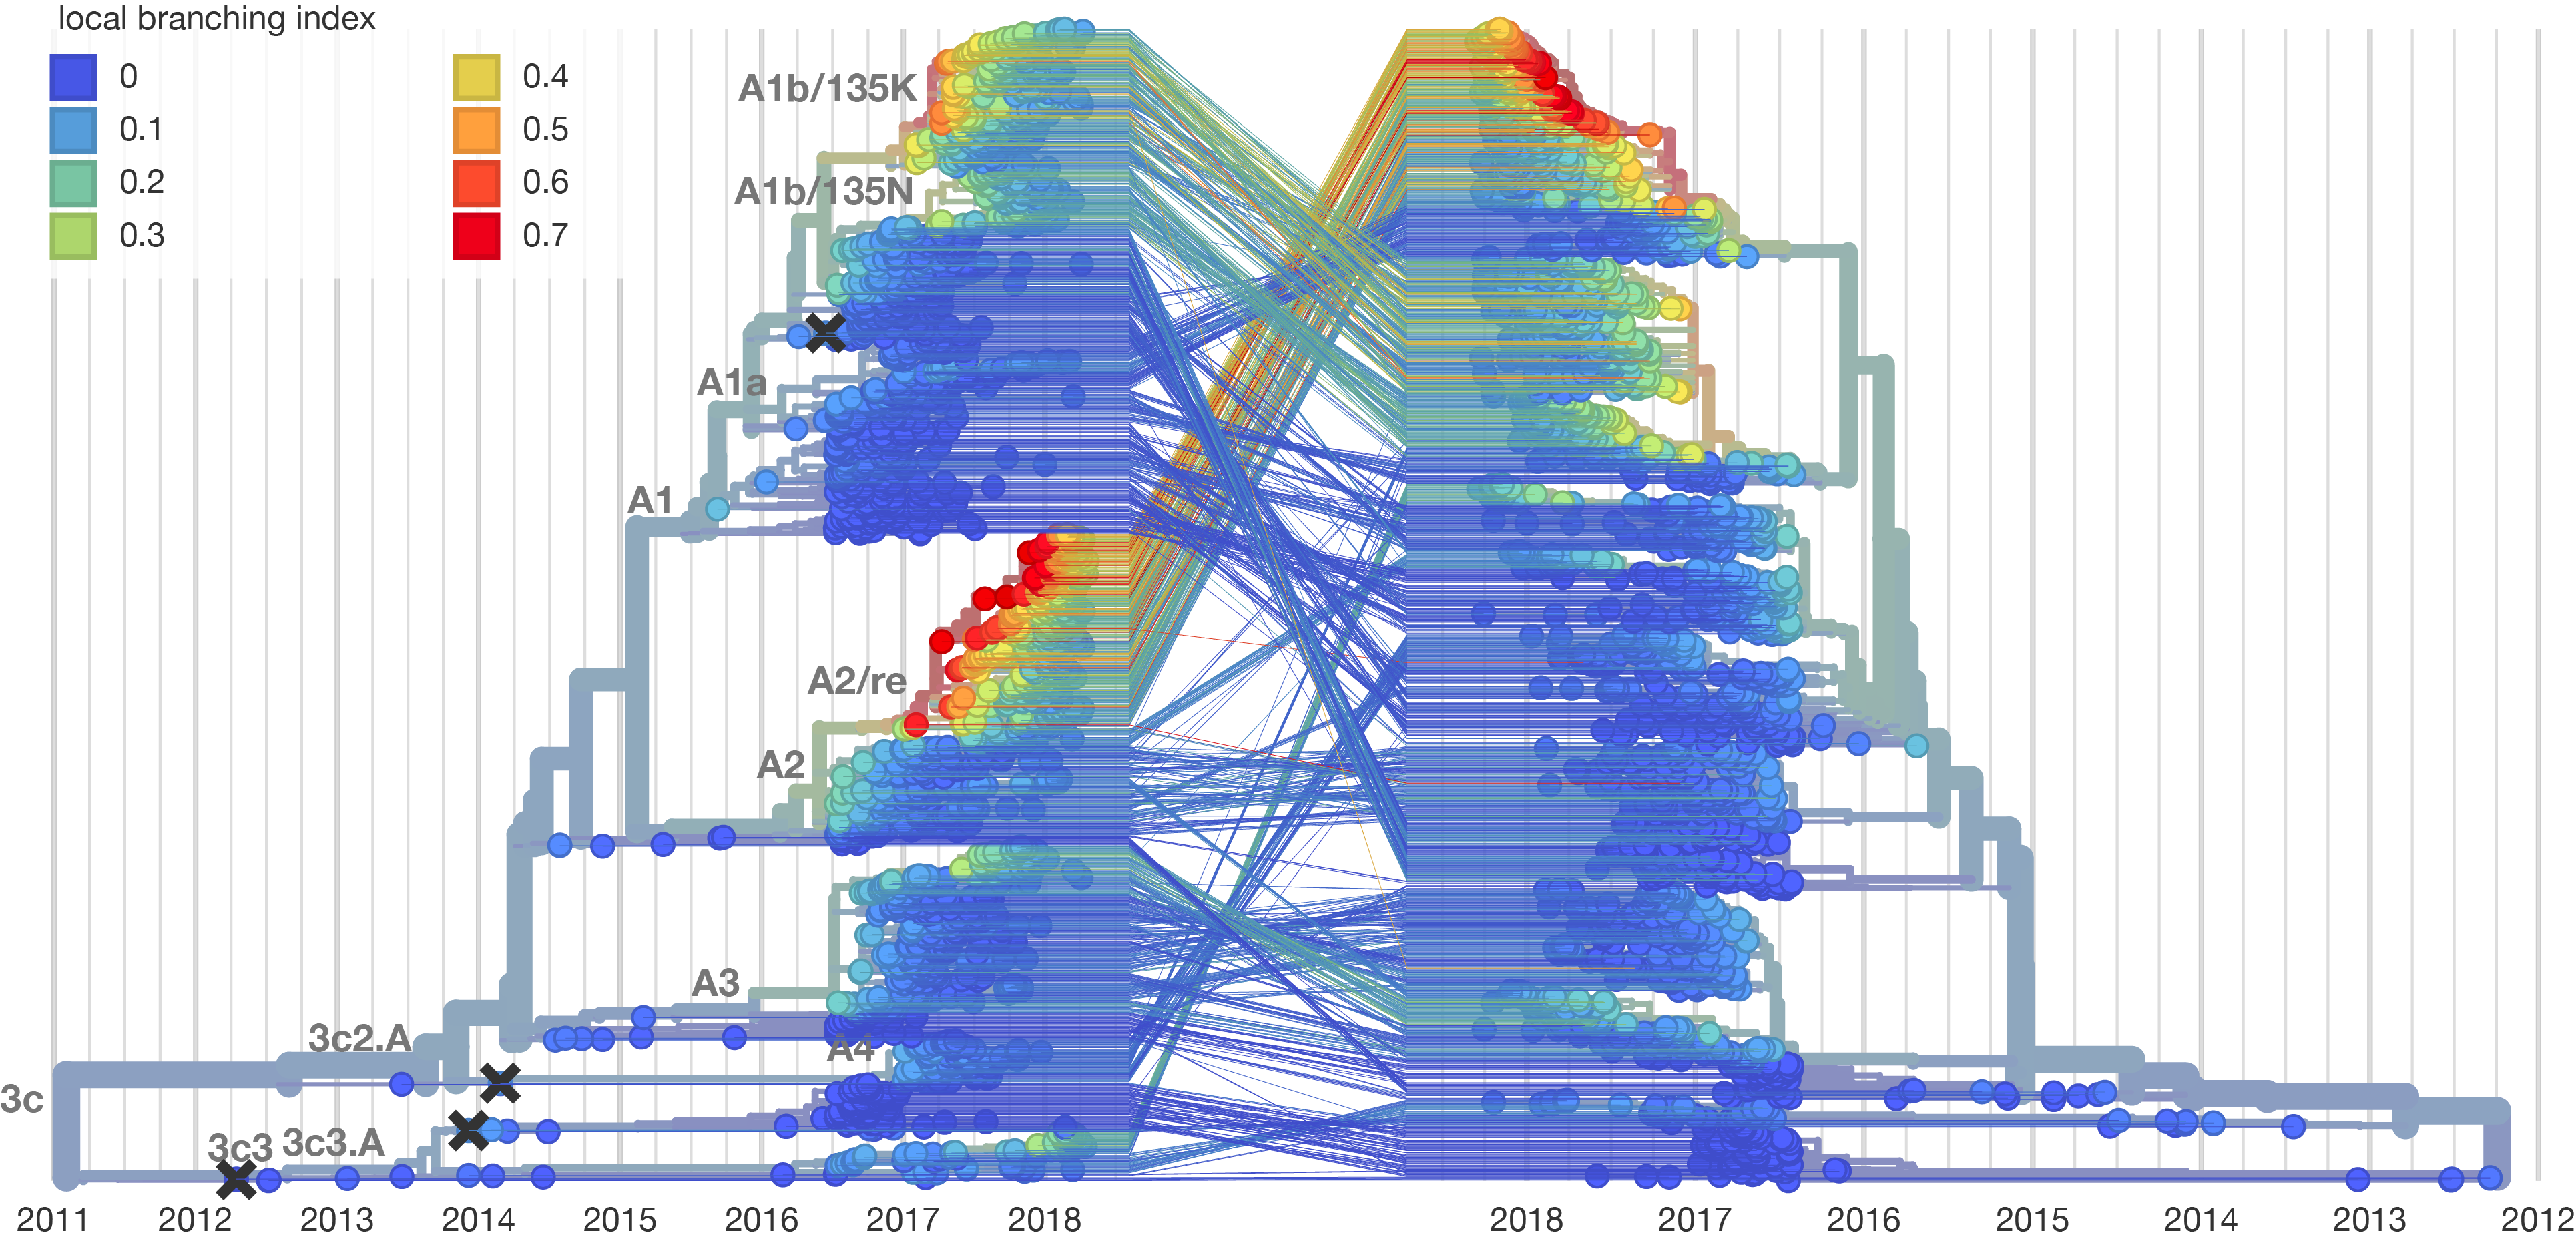
\includegraphics[width=0.85\textwidth]{figures/ha_na_lbi_high_res.png}
    \end{center}
    \caption{Tangle tree matching phylogenetic trees of HA and NA, colored by local branching index (LBI)---a measure that captures rapid expansion of clades. Here, LBI reveals that there is an inflection point where rapid clade growth begins at the same time that A2/re differentiates from A2 in the HA tree. Similarly, LBI is highest in the matched viruses of the NA tree, indicating that the reassortant virus saw much greater success than either of the background viruses from which it arose.}
    \label{sup_fig:lbi}
\end{figure*}

\begin{figure*}[b]
    \begin{center}
    \includegraphics[width=0.99\textwidth]{figures/tangle_all_segments.png}
    \end{center}
    \caption{Tangle trees matching the HA phylogeny (always on left) with the six other non-NA segments. Clade A2 is colored in blue, A1b is colored in yellow, and A2/re is in red. In all segments other than PB1 (top right) A2 and A2/re lie in different parts of the tree in the second segment than in HA, indicating that reassortment has taken place.}
    \label{sup_fig:all_tangle}
\end{figure*}
